\documentclass[11pt, oneside]{article}   	% use "amsart" instead of "article" for AMSLaTeX format
\usepackage{geometry}                		% See geometry.pdf to learn the layout options. There are lots.
\geometry{letterpaper}                   		% ... or a4paper or a5paper or ... 
%\geometry{landscape}                		% Activate for for rotated page geometry
%\usepackage[parfill]{parskip}    		% Activate to begin paragraphs with an empty line rather than an indent
\usepackage{graphicx}				% Use pdf, png, jpg, or eps§ with pdflatex; use eps in DVI mode
								% TeX will automatically convert eps --> pdf in pdflatex		
\usepackage{amssymb}
\usepackage[utf8]{inputenc}
\usepackage{listings}
\usepackage{enumitem}
\usepackage{hyperref}
\usepackage{anyfontsize}
\usepackage{tikz}
\usetikzlibrary{patterns,calc}

\newcommand{\sch}{\lstinline{tpl_sc_handler}}

\title{MSP430X port - basic checkpointing\\design documentation}
\author{David Garriou, Jean-Luc Béchennec}
%\date{}							% Activate to display a given date or no date

\lstset{% general command to set parameter(s)
	basicstyle=\footnotesize\ttfamily,
	backgroundcolor=\color{lightgray!30},
	frame=single, framerule=0pt
}

\begin{document}
\maketitle

\section{Goals and ideas}

\subsection{Consistency}
Our main goal is to keep a system within a coherent state even after a recovery from power loss.
In other words, the kernel execution must be atomic with respect to power loss.

\subsubsection{Consistency of kernel space and user space}

When the system recovers all of its code, user space and kernel space, must be consistent.
\lstinline{OS_VAR} section contains the kernel data structures.
It means that we must not transfer \lstinline{OS_VAR} section to FRAM otherwise the system would recover with two differents (not consistent) states, the last user space state and the latest kernel space state.

We have to save both kernel and user space variables at the same time (during a single checkpoint).

\subsection{Big picture}

Big picture of what to do:
\begin{enumerate}
\item A periodic task, let's call it \lstinline{energy_task}, will check for remaining energy in the super capacitor;
  \begin{enumerate}
  \item user space execution;
  \item remaining energy consists in mesuring VCC voltage (on the terminals of the super capacitor);
  \item if the remaining energy is lower than a defined threshold, we must realize a checkpoint
  \end{enumerate}
\end{enumerate}

\section{Normal MSP430X startup sequence}

The MSP430X startup sequence is as follow:
\begin{enumerate}
\item After a reset, the \lstinline{tpl_reset_handler} executes (see \lstinline{tpl_startup.S} file). It:
	\begin{enumerate}
	\item stops the watchdog timer;
	\item disables the interrupts;
	\item sets up the stack;
	\item calls \lstinline{tpl_continue_reset_handler} C function.
	\end{enumerate}
\item \lstinline{tpl_continue_reset_handler} (see \lstinline{tpl_startup.c} file) does:
	\begin{enumerate}
	\item initialization of the .bss section to 0 (uninitialized variables) and initialization of the .data section by copying the initial values from FRAM (initialized variables)\label{item:bssdatainit}\footnote{Why not use the DMA to do that, it would use less energy};
	\item clock setup by calling \lstinline{tpl_set_mcu_clock}\label{item:clockinit};
	\item initialization of the MPU\label{item:mpuinit}; 
	\item a call to \lstinline{main}\label{item:callmain}.
	\end{enumerate}
\item \lstinline{main} is responsability of the user but usually it:
	\begin{enumerate}
	\item initializes application level devices;
	\item calls \lstinline{StartOS}.
	\end{enumerate}
\item \lstinline{StartOS}:
	\begin{enumerate}
	\item calls \lstinline{tpl_init_machine} that calls;
		\begin{enumerate}
		\item \lstinline{tpl_init_machine_generic} that calls:
			\begin{enumerate}
				\item \lstinline{tpl_init_mpu} which is not implemented yet (and would be redundant with \ref{item:mpuinit}).
			\end{enumerate}
		\item \lstinline{tpl_init_machine_specific} that calls:
			\begin{enumerate}
				\item \lstinline{tpl_set_systick_timer}.
			\end{enumerate}
		\end{enumerate}
	\item calls \lstinline{tpl_start_os} that does a system call to \lstinline{tpl_start_os_service} that.
		\begin{enumerate}
		\item calls \lstinline{tpl_init_os};
		\item calls \lstinline{tpl_enable_counters};
		\item calls \lstinline{StartupHook} if any;
		\item calls \lstinline{tpl_start_scheduling}.
		\end{enumerate}
		when returning a task is schedule.
	\end{enumerate}
\end{enumerate}

\section{Modified sequence to restore a checkpoint}\label{sec:checkpointrestore}

Following items shall be modified when restarting from a checkpoint:

\begin{itemize}
\item item \ref{item:bssdatainit} should be replaced by a copy from the checkpoint data in FRAM to SRAM.
\item item \ref{item:clockinit} should use the replaced by an init with the clock frequency when the checkpoint was done. This can be done by having a variable (in .data segment) to store the clock frequency so that it would restored as part of the checkpoint data.
\item item \ref{item:callmain} should be replaced by a call to a mandatory function used to initialize the devices for the application (UART for instance) and to a new service, let's call it \lstinline{RestartOS}. \lstinline{RestartOS} would:
	\begin{enumerate}
	\item Call \lstinline{tpl_init_machine};
	\item Call \lstinline{tpl_restart_os} that does a system call to \lstinline{tpl_restart_os_service} that does a \lstinline{tpl_start}. \lstinline{tpl_start} moves the highest priority task from the ready list to the elected slot of \lstinline{tpl_kern}. Conditions shall be \lstinline{NEED_SWITCH} true and \lstinline{NEED_SAVE} false.  
	\end{enumerate}
\end{itemize}

When returning from the \lstinline{RestartOS} service, the highest priority task is scheduled and the system continues execution.

A boolean variable stored in FRAM, let's call it \lstinline{tpl_checkpoint_available}, shall be used to select, when true, the modified sequence instead of the normal one.

\section{Checkpointing}\label{sec:checkpointing}

A new service is necessary, let's call it \lstinline{Hibernate}. When called, \lstinline{Hibernate}, terminates the caller. It copies the SRAM to the FRAM (checkpoint), stops the Systick, stops application interrupts (a user function shall be provided for that), programs the RTC to emit an interrupt every x seconds, enables interrupts and goes in LPM3. 

The RTC ISR check the voltage of the MCU. If it is above a threshold (\lstinline{RESUME_FROM_}\-\lstinline{HIBERNATE_THRESHOLD}), it exists from LPM3. If this never happens, after a while, the MCU will power off. When in the future the MCU restart, what is described in section \ref{sec:checkpointrestore} applies.  

If \lstinline{Hibernate} resumes because the RTC ISR exited from LPM3 then it disables interrupt, starts application interrupts, starts the Systick, stop the RTC. It calls \lstinline{tpl_start} to elect the highest priority task and returns.

In addition, a periodic basic task, \lstinline{energy_task} checks (every 5 seconds ? more ?) the voltage. If the voltage drops below a threshold (\lstinline{HIBERNATE_THRESHOLD}), \lstinline{energy_task} calls \lstinline{Hibernate} (and terminates):

\begin{lstlisting}[language=C]
TASK(energy_task)
{
  uint16 voltage = readPowerVoltage();
  if (voltage < HIBERNATE_THRESHOLD) {
    Hibernate();
  }
  else {
    TerminateTask();
  }
}
\end{lstlisting}

\lstinline{HIBERNATE_THRESHOLD} shall be chosen so that the worst voltage drop between 2 executions of \lstinline{energy_task} plus the voltage drop due to checkpointing is lower than the threshold.

\lstinline{HIBERNATE_THRESHOLD} shall be lower than \lstinline{RESUME_FROM_}\-\lstinline{HIBERNATE_THRESHOLD}.

\subsection{OIL modifications}

An OS attribute is added:

\begin{lstlisting}
BOOLEAN CHECKPOINT = FALSE;
\end{lstlisting}

\subsection{DMA}

Both checkpoint save and checkpoint restore are done using the DMA. The MSP430FR5994 has 6 DMA channels. Channel 0 is used. The block transfer mode is used. DMA is triggered by software. It copies the whole content of the SRAM (8kB, from 0x1C00 to 0x3BFF) to the FRAM. It would be safer to use double buffering because if a checkpoint cannot complete before the loss of power for any reason, the previous checkpoint will not be corrupted. An int variable in FRAM with value equal to 0, 1 or -1 is used to select the buffer. Let's call it \lstinline{tpl_checkpoint_buffer}. If the value is -1, no checkpoint is saved. This is the initial value. If value is 0 a checkpoint is saved in buffer 0 and if value is 1, a checkpoint is saved in buffer 1. Saving a checkpoint would be as follow: 

\begin{lstlisting}
int buffer = (tpl_checkpoint_buffer + 1) & 1;
tpl_save_checkpoint(buffer);
tpl_checkpoint_buffer = buffer;
\end{lstlisting}

If power is lost during the \lstinline{tpl_save_checkpoint} function, \lstinline{tpl_checkpoint_buffer} is not updated and the checkpoint is not committed. 

The content of \lstinline{tpl_checkpoint_buffer} is used to select the normal startup described at section \ref{sec:normalstart} or the startup from a checkpoint described at section \ref{sec:checkpointrestore}.

\begin{lstlisting}
#define OS_START_SEC_CONST_16BIT
#include "tpl_memmap.h"
static CONST(sint16, OS_CONST) NO_CHECKPOINT = -1;
#define OS_STOP_SEC_CONST_16BIT
#include "tpl_memmap.h"

#define OS_START_SEC_NON_VOLATILE_VAR_16BIT
#include "tpl_memmap.h"
VAR(sint16, OS_VAR) tpl_checkpoint_buffer = -1;
#define OS_STOP_SEC_NON_VOLATILE_VAR_16BIT
#include "tpl_memmap.h"

if (tpl_checkpoint_buffer == NO_CHECKPOINT) {
  /* normal startup */
}
else {
  /* startup from checkpoint */
}
\end{lstlisting}

The 2 buffers are located above the 64kB limit, at the end of the FRAM for instance. The first one from 0x040000 to 0x041FFFh and the second one from 0x042000 to 0x043FFFh.
The SRAM starts at address 0x001C00 and ends at address 0x003BFF.

The function to save the SRAM to a buffer using the DMA has to be written in assembly because writing to start address and end address registers shall be done using extended instructions when address is above the 64kB limit:

\begin{lstlisting}
#include "tpl_assembler.h"

.equ SRAM_START      0x1C00
.equ BUFFER0_START   0x040000
.equ BUFFER1_START   0x042000
.equ CHECKPOINT_SIZE 0x1000 /* 4k words  */
.equ START_TRANSFER  0x1F11 /* see below */

/*
 * tpl_save_checkpoint
 * Argument is the buffer: 0 or 1
 */
.global tpl_save_checkpoint
.type   tpl_save_checkpoint, %function

tpl_save_checkpoint:

  mov    #0, &DMACTL0  /* DMA Channel 0 is triggered by software (DMAREQ) */
  mov    #SRAM_START, &DMA0SA      /* Source address is SRAM address      */
  tst    REG_RETARG
  jnz    buffer1
  movx.a #BUFFER0_START, &DMA0DA   /* Destination address is buffer 0     */
  jmp    cont
buffer1:
  movx.a #BUFFER1_START, &DMA0DA   /* Destination address is buffer 1     */
cont:
  mov    #CHECKPOINT_SIZE, &DMA0SZ /* Size of the transfer                */
  
  mov    #START_TRANSFER, &DMA0CTL /* Start the transfer                  */
  ret
\end{lstlisting}

\subsubsection*{\lstinline{START_TRANSFER} explanation}

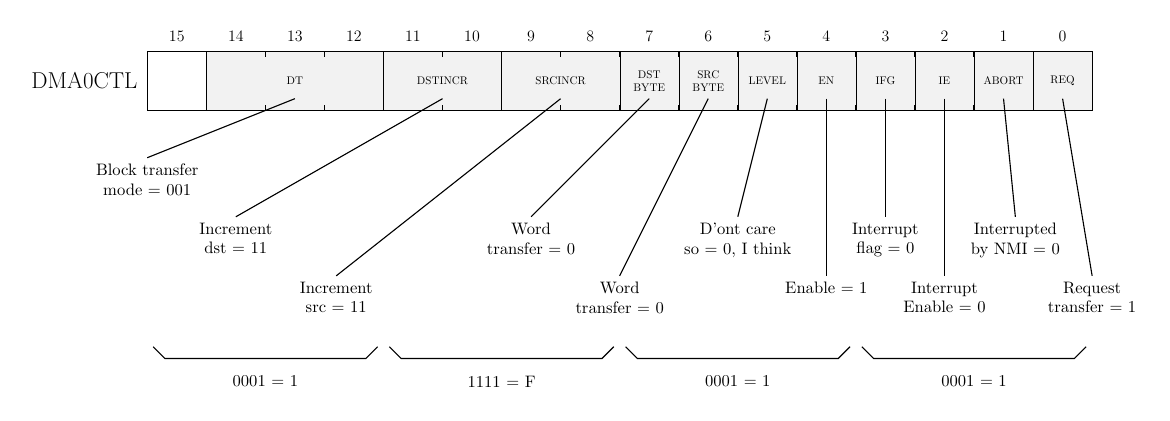
\begin{tikzpicture}[scale=.75,every node/.style={scale=0.4}]
\tikzstyle{comm}=[scale=1.5,anchor=north,align=center]

\draw[ultra thin,fill=gray!10] (1,0) rectangle ++(3,1);
\node at (2.5,.5) {DT};

\draw[ultra thin,fill=gray!10] (4,0) rectangle ++(2,1);
\node at (5,.5) {DSTINCR};

\draw[ultra thin,fill=gray!10] (6,0) rectangle ++(2,1);
\node at (7,.5) {SRCINCR};

\draw[ultra thin,fill=gray!10] (8,0) rectangle ++(1,1);
\node[align=center] at (8.5,.5) {DST\\BYTE};

\draw[ultra thin,fill=gray!10] (9,0) rectangle ++(1,1);
\node[align=center] at (9.5,.5) {SRC\\BYTE};

\draw[ultra thin,fill=gray!10] (10,0) rectangle ++(1,1);
\node[align=center] at (10.5,.5) {LEVEL};

\draw[ultra thin,fill=gray!10] (11,0) rectangle ++(1,1);
\node[align=center] at (11.5,.5) {EN};

\draw[ultra thin,fill=gray!10] (12,0) rectangle ++(1,1);
\node[align=center] at (12.5,.5) {IFG};

\draw[ultra thin,fill=gray!10] (13,0) rectangle ++(1,1);
\node[align=center] at (13.5,.5) {IE};

\draw[ultra thin,fill=gray!10] (14,0) rectangle ++(1,1);
\node[align=center] at (14.5,.5) {ABORT};

\draw[ultra thin,fill=gray!10] (15,0) rectangle ++(1,1);
\node[align=center] at (15.5,.5) {REQ};

\draw (0,0) rectangle (16,1);
\foreach \x in {1,2,...,15} {
  \draw (\x,0) -- ++(0,.1);
  \draw (\x,1) -- ++(0,-.1);
}
\foreach \x in {15,14,...,0} {
  \node[anchor=south] at ($(15.5-\x,1.1)$) {\Large\x};
}
\node[anchor=east] at (-0.1,.5) {\huge DMA0CTL};

\draw (2.5,.2) -- (0,-.8) node[comm] {Block transfer\\mode = 001};
\draw (5,.2) -- (1.5,-1.8) node[comm] {Increment\\dst = 11};
\draw (7,.2) -- (3.2,-2.8) node[comm] {Increment\\src = 11};
\draw (8.5,.2) -- (6.5,-1.8) node[comm] {Word\\transfer = 0};
\draw (9.5,.2) -- (8,-2.8) node[comm] {Word\\transfer = 0};
\draw (10.5,.2) -- (10,-1.8) node[comm] {D'ont care\\so = 0, I think};
\draw (11.5,.2) -- (11.5,-2.8) node[comm] {Enable = 1};
\draw (12.5,.2) -- (12.5,-1.8) node[comm] {Interrupt\\flag = 0};
\draw (13.5,.2) -- (13.5,-2.8) node[comm] {Interrupt\\Enable = 0};
\draw (14.5,.2) -- (14.7,-1.8) node[comm] {Interrupted\\by NMI = 0};
\draw (15.5,.2) -- (16,-2.8) node[comm] {Request\\transfer = 1};

\foreach \x in {0,4,8,12} {
  \draw ($(\x+.1,-4)$) -- ++(.2,-.2) -- ++(3.4,0) -- ++(.2,.2);
}
\node[comm] at (2,-4.4) {0001 = 1};
\node[comm] at (6,-4.4) {1111 = F};
\node[comm] at (10,-4.4) {0001 = 1};
\node[comm] at (14,-4.4) {0001 = 1};
\end{tikzpicture}

\section{New services}

\subsection{Service \lstinline{RestartOS}}

\subsection{Service \lstinline{Hibernate}}

\section{Peripherals}

Specific code for peripherals re-initialization.
TODO
They have to be re-initialized before main call.


\end{document}  

